\documentclass[10pt,a4paper]{article}
\usepackage[utf8]{inputenc}
\usepackage{amsmath}
\usepackage{amsfonts}
\usepackage{amssymb}
\usepackage{tikz}
\usepackage{graphicx}
\author{James Lee}
\title{13th Assignment of Computational Physics}
\begin{document}
	\maketitle
	\begin{abstract}
		In this report I present to you the numerical solution to Problem 5.3.
	\end{abstract}
	\section{Introduction}
	In mathematics, Laplace's equation is a second-order partial differential equation named after Pierre-Simon Laplace who first studied its properties. This is often written as:
	\begin{equation}
	 \nabla^2 \varphi = 0  \qquad\mbox{or}\qquad \Delta\varphi = 0
	\end{equation}
	Laplace's equation and Poisson's equation are the simplest examples of elliptic partial differential equations. The general theory of solutions to Laplace's equation is known as potential theory. The solutions of Laplace's equation are the harmonic functions, which are important in many fields of science, notably the fields of electromagnetism, astronomy, and fluid dynamics, because they can be used to accurately describe the behavior of electric, gravitational, and fluid potentials. In the study of heat conduction, the Laplace equation is the steady-state heat equation.\\
	Our problem is strictly restricted in 2 dimension plane, the PDE can be written as:
	\begin{align}
	\frac{\partial^2\psi}{\partial x^2} + \frac{\partial^2\psi}{\partial y^2} \equiv \psi_{xx} + \psi_{yy} = 0
	\end{align}
	The boundary condition is:
	\begin{align}
	& V|_{x=3}=V|_{y=3}=V|_{x=-3}=V|_{y=-3}=0\\
	& V|_{x=1,|y|<1}=-1\\
	& V|_{x=-1,|y|<1}=1
	\end{align}
	In the following discussions, I will exploit numerical methods to study its solution.
	
	\section{Main Contents}
	\subsection{Jacobi Method}
	Jacobi method is a powerful method to solve a PDE numerically. In order to solve for the final function, one need to crystalize the space at first. Then one guesses a solution that satisfies the boundary condition, and uses:
	\begin{equation}
	V_{n+1}(i,j)=\frac{V_{n}(i-1,j)+V_{n}(i,j-1)+V_{n}(i+1,j)+V_{n}(i,j+1)}{4}
	\end{equation}
	to obtain a better solution. One should continue this iteration until the solution becomes satisfying.\\
	By using Jacobi method, I can obtain the final solution shown in the plots:
	\begin{figure}[htbp]
		\centering
		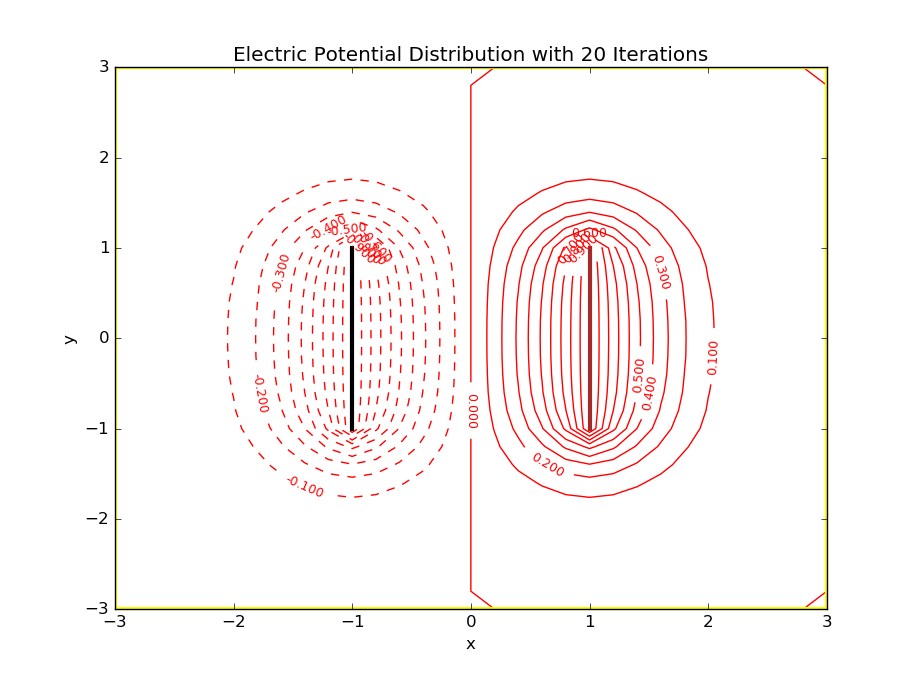
\includegraphics[width=5in]{laplace_2.png}
		\caption{Numerical Solution with 20 iterations}
	\end{figure}
	\begin{figure}[htbp]
		\centering
		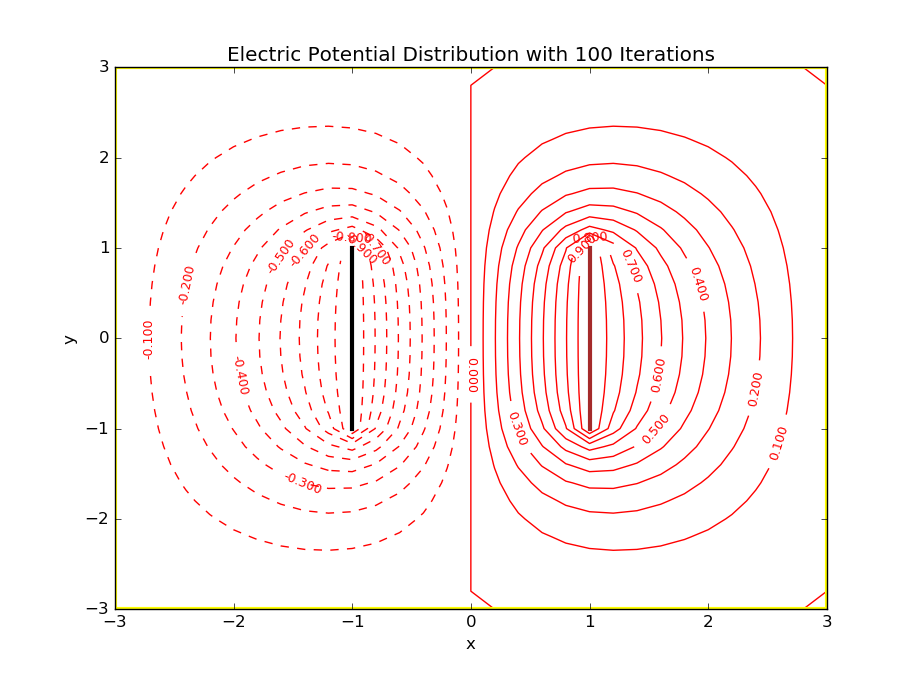
\includegraphics[width=5in]{laplace_1.png}
		\caption{Numerical Solution with 100 iterations}
	\end{figure}
	\begin{figure}[htbp]
		\centering
		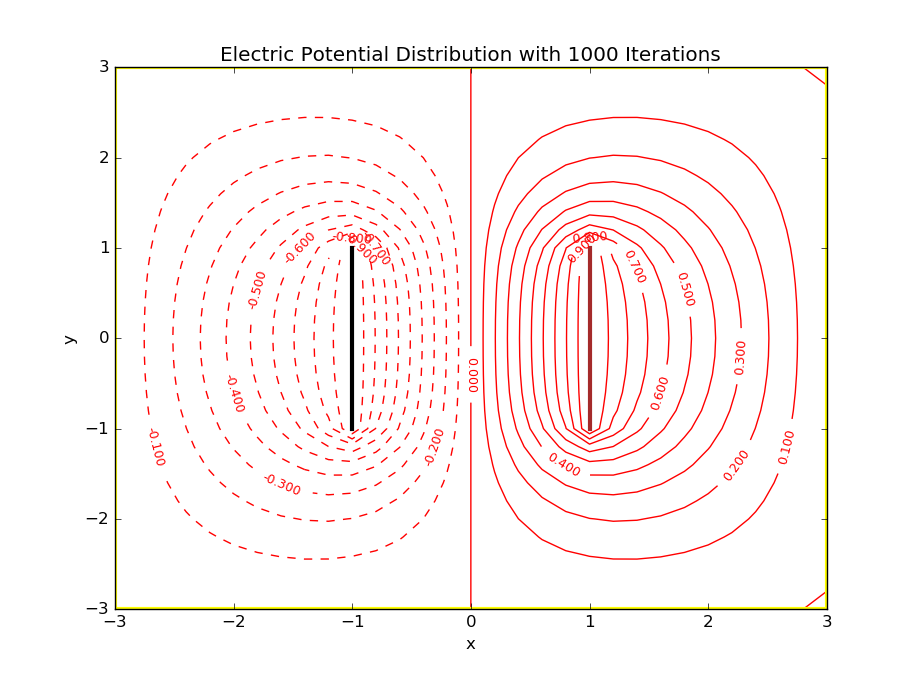
\includegraphics[width=5in]{laplace_3.png}
		\caption{Numerical Solution with 1000 iterations}
	\end{figure}
	As we can see in the plots, the final result quite agrees with our common sense. When iterations reaches 100 times, more iterations do not change the solution extraodinarily. 
	
	\subsection{Analysis of Efficiency of Different Algorithms}
	It is not difficult to show that SOR method can easily obtain the same results faster than this.
	But how can we analyze this problem quantitatively? I have written a program that can examine the iteration-steps correspondence with these two algorithms, the results are shown in figure.4.\\
		\begin{figure}[htbp]
			\centering
			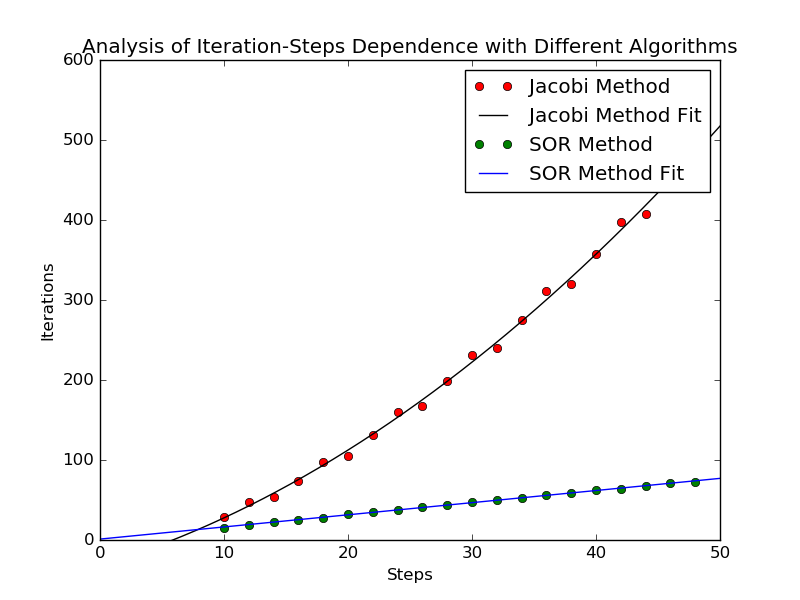
\includegraphics[width=5in]{laplace_4.png}
			\caption{Analysis of Iteration-Steps Dependence with Different Algorithms}
		\end{figure}
	The fit curves in the plot are obtained through regression analysis. It was shown that SOR algorithms have a $n\propto L$ correspondence, while the Jacobi methods have a $n\propto L^2$ correspondence.\\
	Therefore, we conclude that the SOR method is more efficient than Jacobi method.
	
	\section*{Acknowledgement}
	When tackling this assignment, I benefitted a lot from the valuable programs by Chen Yangyao and Zhang Qi. I would like to thank them for pointing out several syntax errors I made, also, for their willingness to discuss with me.
	
	\begin{thebibliography}{99}
		\bibitem{}Hunter J, the Matplotlib Documentation, 2016
		\bibitem{}Giordano N.J, Nakanishi H, Computational Physics, Pearson Education, 2007
	\end{thebibliography} 
\end{document}